\documentclass[french]{standalone}
\usepackage{babel}
\usepackage{tkz-fct}
\usepackage{tkz-euclide}
\usepackage{color}
\usepackage{numprint}
\usepackage{amsmath}
\renewcommand*\familydefault{\sfdefault}
\usepackage{sansmath}
\sansmath
\definecolor{gray75}{gray}{0.75}

\begin{document}
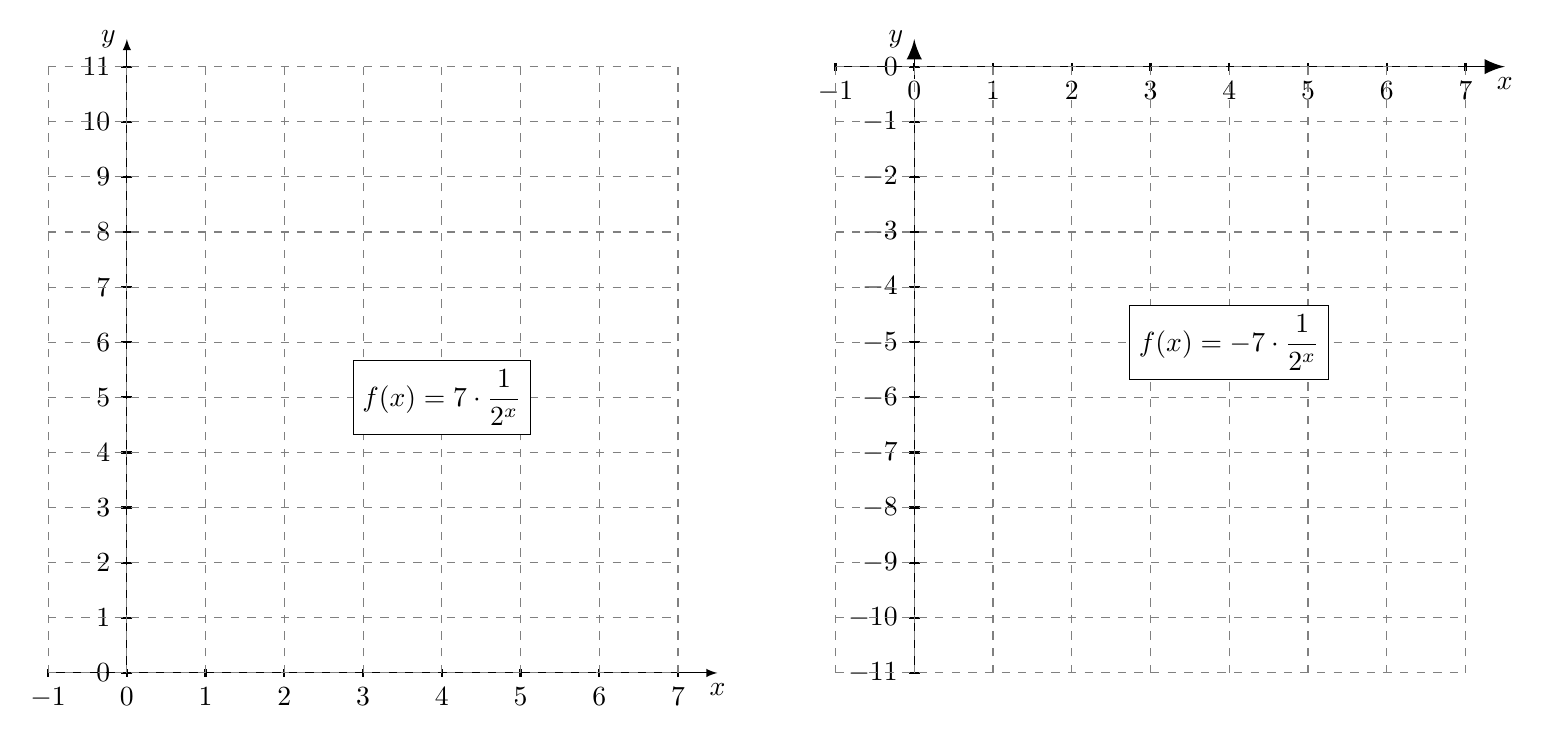
\begin{tikzpicture}[yscale=0.7, xscale=1]
\tkzInit[xmin=-1,xmax=7,ymin=0,ymax=11, ystep=1, xstep=1]
\tkzAxeY
\tkzDrawX
\tkzLabelX
   \begin{scope}[dashed]
     \tkzGrid
   \end{scope}
   \tkzFct[domain=-1:7,line width=1.5pt]{(7*exp(-log(2)*x))}
   \tkzText[draw,fill=white](4,5){$f(x)=7\cdot\dfrac{1}{2^{x}}$}

\begin{scope}[xshift=10cm, yshift=11cm]
\tkzInit[xmin=-1,xmax=7,ymin=-11,ymax=0, ystep=1, xstep=1]
\tkzAxeY
\tkzDrawX
\tkzLabelX

   \begin{scope}[dashed]
     \tkzGrid
   \end{scope}
      \tkzFct[domain=-1:7,line width=1.5pt]{(-7*exp(-log(2)*x))}

   \tkzText[draw,fill=white](4,-5){$f(x)=-7\cdot\dfrac{1}{2^{x}}$}

\end{scope}
\end{tikzpicture}
\end{document}
